%Miriam Clustering

\section{Clustering with RapidMiner}

RapidMiner has different Modules for Clustering already implemented. We apply the k-Means algorithm with mixed measure (euclidean).

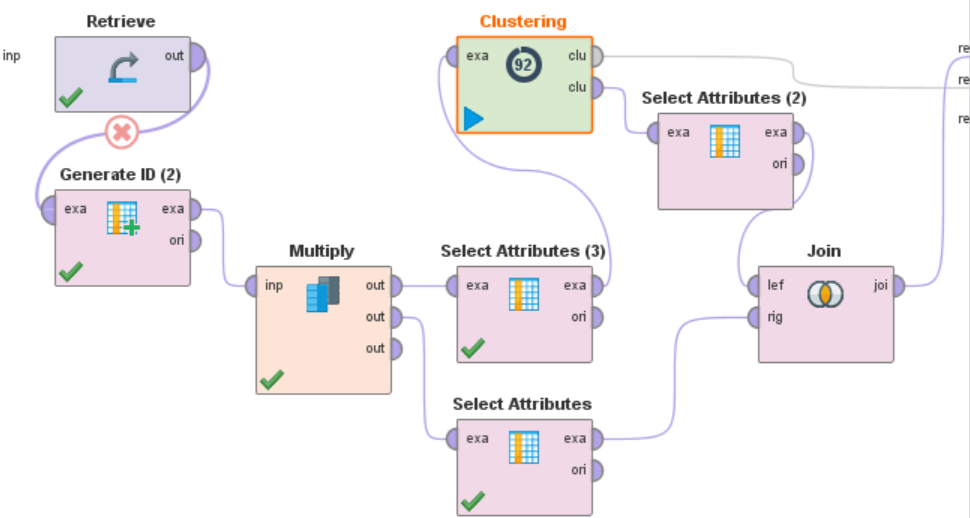
\includegraphics[width=0.9\textwidth]{../Miriam-RapidMiner/ClusteringRapid.PNG}


The Process does the following steps:
\begin{description}
	\item[Retrieve] This Block gives the data in the process. For the comparison at the end we also retrieve the original data.
	\item[Nominal to Numerical] This changes the nominal data to numerical data, so that we can apply PCA in the next step
	\item[PCA] Here we apply the PCA reduction to the data with a variance threshold $0.95$ \colorbox{red}{where?}
	\item[Clustering] Here the number of Clusters has to be fixed. We decided, that 10 runs should be enough. We can choose between differen measure types and tried mixed euclidean and squared euclidean distance
	\item[Select Attribute] Here we just pick the Strata data for comparing with the clustering
	\item[Join] For comparing the Clustering and the Strata we join the two filtered data sets at the ID
\end{description}

\subsection{Original Data}

\subsubsection{Searching for 6 Cluster}
Applying this process to the original data you can see without alignment of strata and cluster, that the distribution of cluster and strata is not close to the same.

\ref{fig:OrgDist}. 
\begin{figure}
\centering
\begin{subfigure}{.5\textwidth}
  \centering
  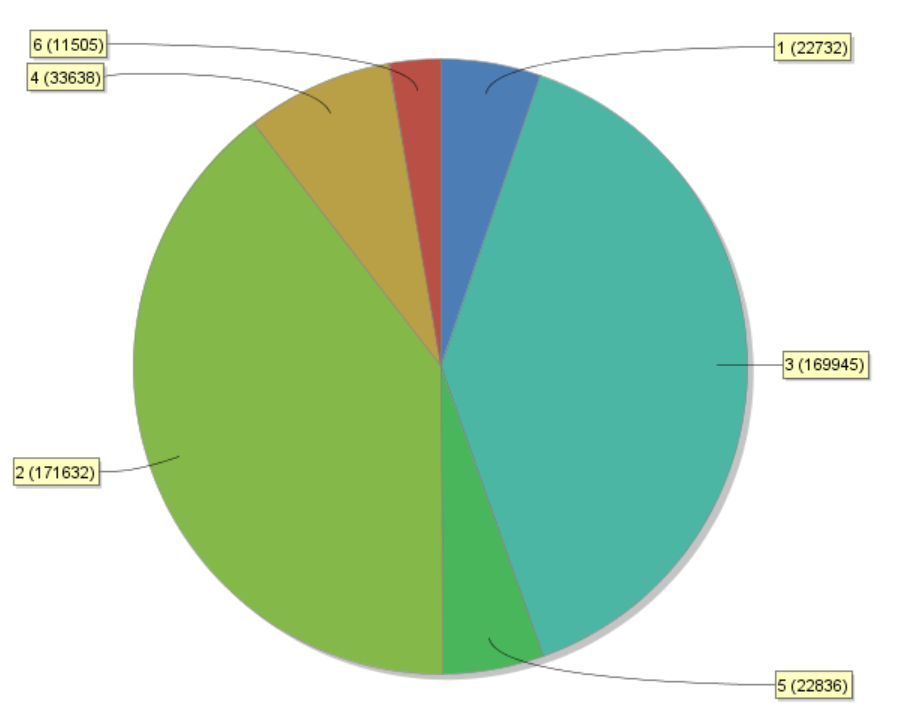
\includegraphics[width=.4\linewidth]{../Miriam-RapidMiner/ClusterPCAOrigRapidStrata.PNG}
  \caption{Strata}
  \label{fig:OrgSt}
\end{subfigure}%
\begin{subfigure}{.5\textwidth}
  \centering
  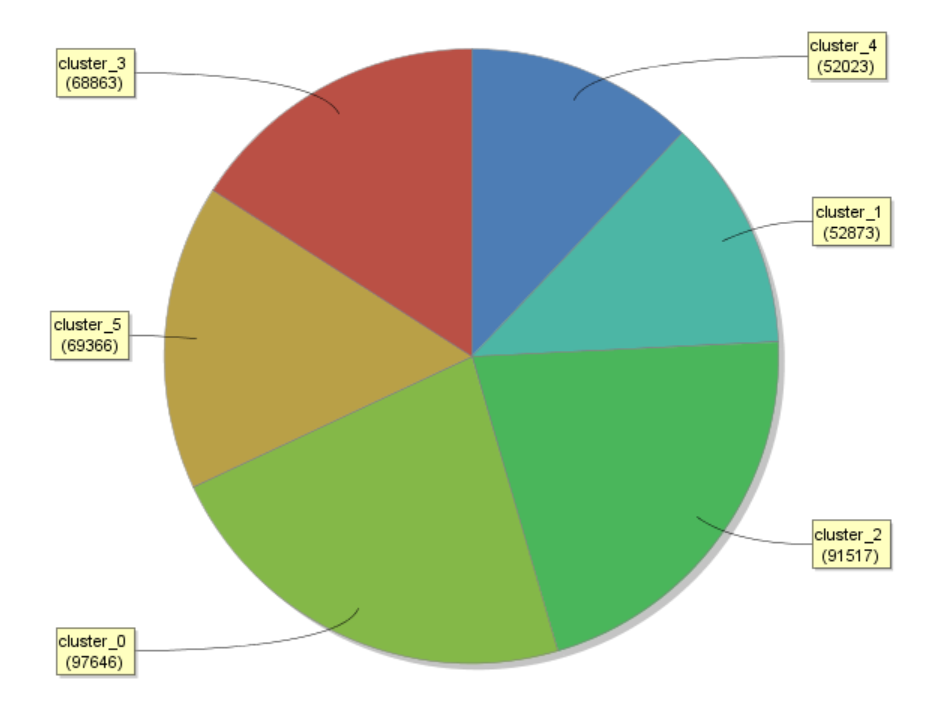
\includegraphics[width=.4\linewidth]{../Miriam-RapidMiner/ClusterPCAOrigRapidCluster.PNG}
  \caption{Cluster}
  \label{fig:OrgCl}
\end{subfigure}
\caption{Distribution of original data}
\label{fig:OrgDist}
\end{figure}

\subsubsection{Searching for 3 Cluster}

The next idea is, that there are maybe just 3 obvious cluster to see and contain two 2 strata.

\subsubsection{Applying on original data}

For a clustering of 3 clusters we get a distributions that are complete different.\ref{fig:OrgDist}
\begin{figure}[h]
\centering
\begin{subfigure}{.5\textwidth}
  \centering
  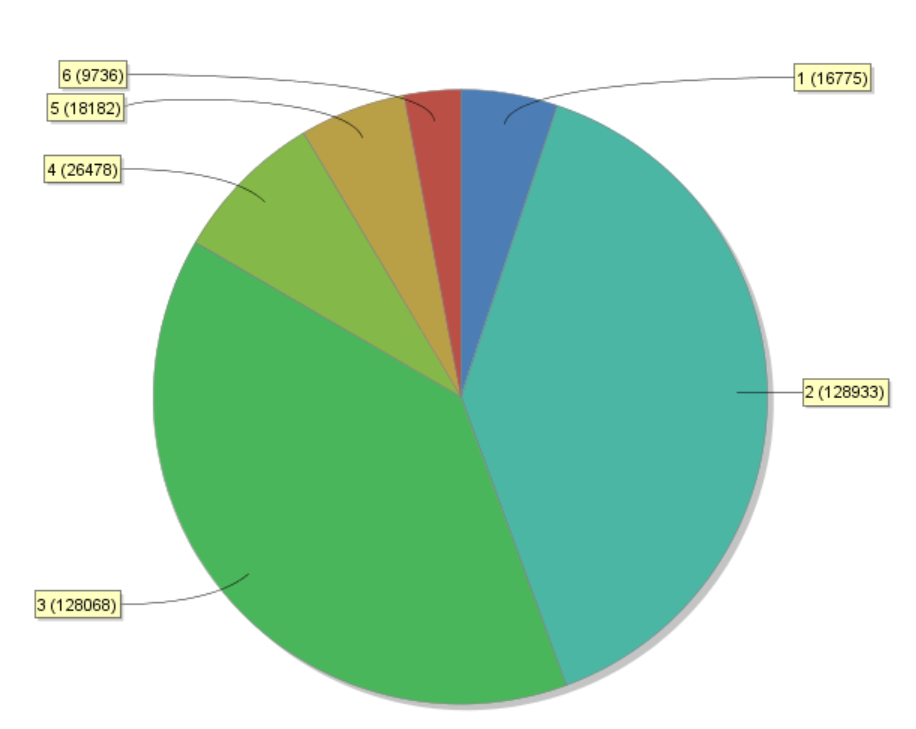
\includegraphics[width=.4\linewidth]{../Miriam-RapidMiner/ClusterOrigRapidStrata2Cluster.PNG}
  \caption{Strata}
  \label{fig:OrgSt}
\end{subfigure}%
\begin{subfigure}{.5\textwidth}
  \centering
  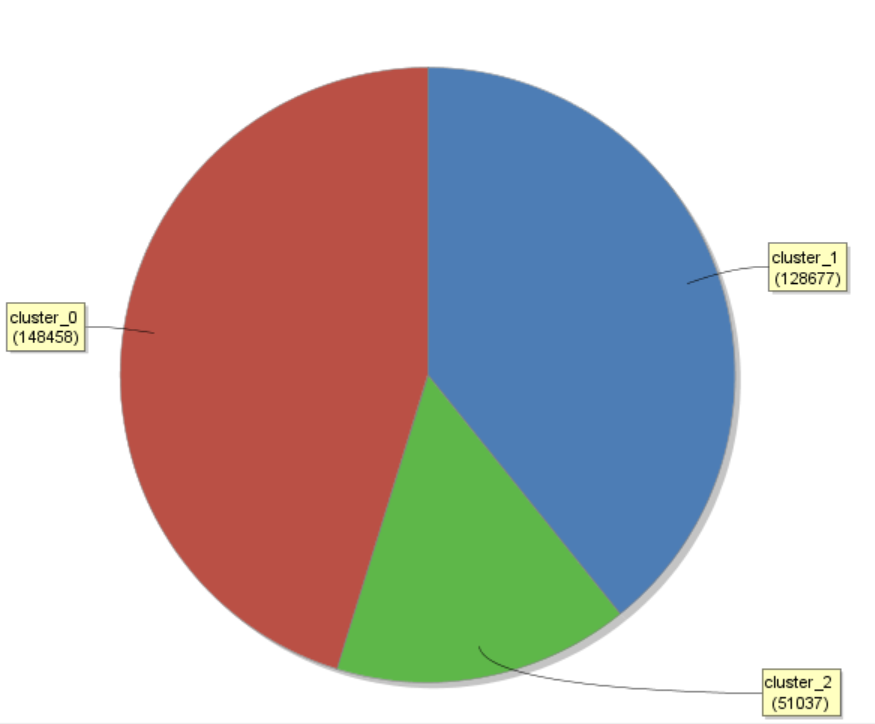
\includegraphics[width=.4\linewidth]{../Miriam-RapidMiner/ClusterOrigRapidCluster2Cluster.PNG}
  \caption{Cluster}
  \label{fig:OrgCl}
\end{subfigure}
\caption{Distribution of original data}
\label{fig:OrgDist}
\end{figure}

Also the distribution in the strata groups of the clustering shows, that there is no real connection of strata and the clustering.
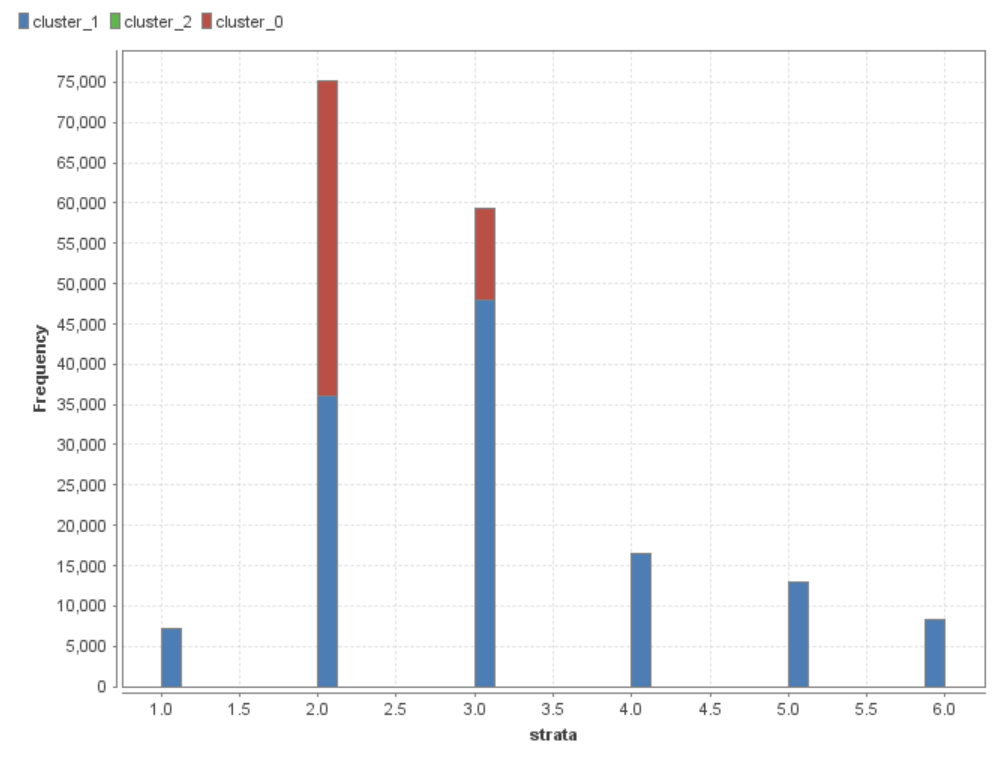
\includegraphics[width=0.9\textwidth]{../Miriam-RapidMiner/ClusterOrigRapidDistribution2Cluster.PNG}

\subsection{Combined Data}

Because of the not really convincing result of the clustering like above we had the idea to combine for every ID the different pathes in one big vector. This garants us, that one person just can be in one cluster aswell. The idea is to sum up all pathes in one big vector.
\subsubsection{Code}
%hier darfst du dich gerne verewigen Timo. Gerne auch vorher und nachher noch mehr schreiben. Titel darf auch geändert werden
% boa das ist voll liep un soo weischt :D

Instead of simple IDs for every person we expand the parsing by using a data encapsulating in a class called \texttt{Person}. This class stores the ID, the parameters defining a person %TODO: ref zu code basics
, and all movements from that person.\\
Then we are able to compute the following vector, with 848 entries, for further usage, that combines all movements of the person:
$$\underbrace{\#o_1, \dots, \#o_{413}, \#d_1, \dots, \#d_{413}}_{2\cdot 413} ,
 \underbrace{\mathit{AM}, \mathit{MD}, \mathit{PM}, \mathit{MN}}_{4}, 
 \underbrace{\#r_1, \dots, \#r_7}_{7}, 
 \underbrace{\#\mathit{MoT}_1, \dots, \#\mathit{MoT}_7}_{7}, 
 \underbrace{\mathit{SD}, \mathit{SS}, \mathit{G}, \mathit{A}}_{4}$$
with the following abbreviations ($1 \le i \le 413$, $0 \le j \le 7$):
\begin{multicols}{2}
\begin{itemize}
	\item[$o_i$:]  the $i$-th origin data point
	\item[$d_i$:]  the $i$-th destination data point
	\item[$\mathit{AM}$:] movements at time stamp AM
	\item[$\mathit{MD}$:] movements at time stamp MD
	\item[$\mathit{PM}$:] movements at time stamp PM
	\item[$\mathit{MN}$:] movements at time stamp MN
	\item[$r_j$:] the $j$-th reason
	\item[$\mathit{MoT}_j$:] the $j$-th mean of transportation
	\item[$\mathit{SD}$:] sum of all durations
	\item[$\mathit{SS}$:] sum of all distances
	\item[$\mathit{G}$:] the gender
	\item[$\mathit{A}$:] the age
\end{itemize}
\end{multicols}

\subsubsection{Searching for 6 Clusters}
Applying the process with maximal 100 steps on the data gives us the following results.

Like above we check first the total distribution of strata and clusters with a pie. You already see, that it is not the 
\begin{figure}[h]
\centering
\begin{subfigure}{.5\textwidth}
  \centering
  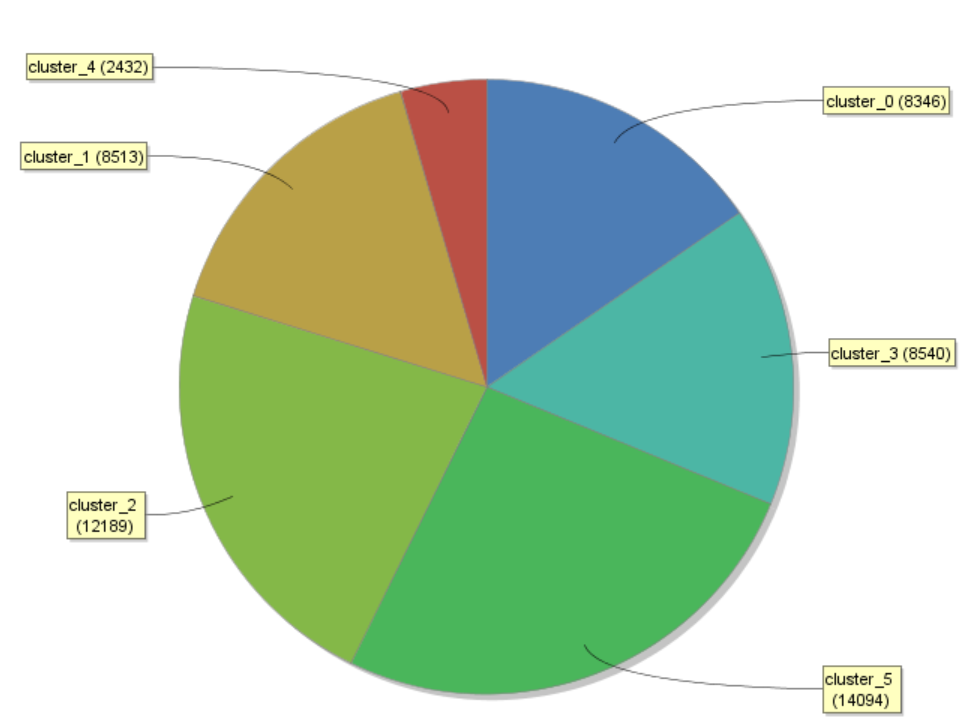
\includegraphics[width=.4\linewidth]{../Miriam-RapidMiner/vectorclusteringcluster.PNG}
  \caption{Strata}
  \label{fig:OrgSt}
\end{subfigure}%
\begin{subfigure}{.5\textwidth}
  \centering
  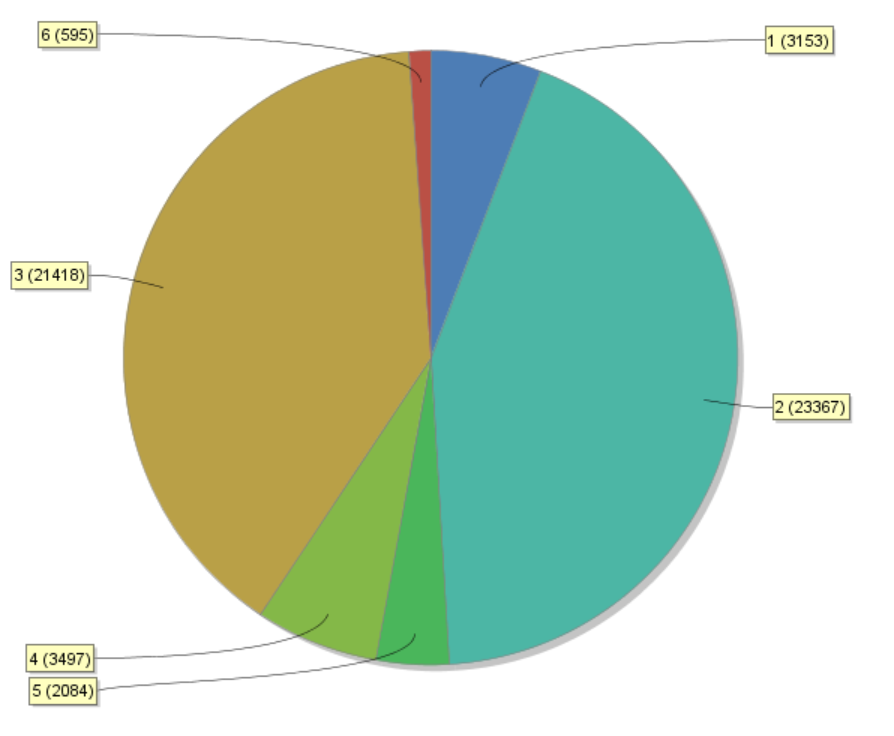
\includegraphics[width=.4\linewidth]{../Miriam-RapidMiner/vectorclusteringstrata.PNG}
  \caption{Cluster}
  \label{fig:OrgCl}
\end{subfigure}
\caption{Distribution of original data}
\label{fig:OrgDist}
\end{figure}

Also the distribution in the strata groups of the clustering shows, that there is not really a connection of strata and the clustering to see.
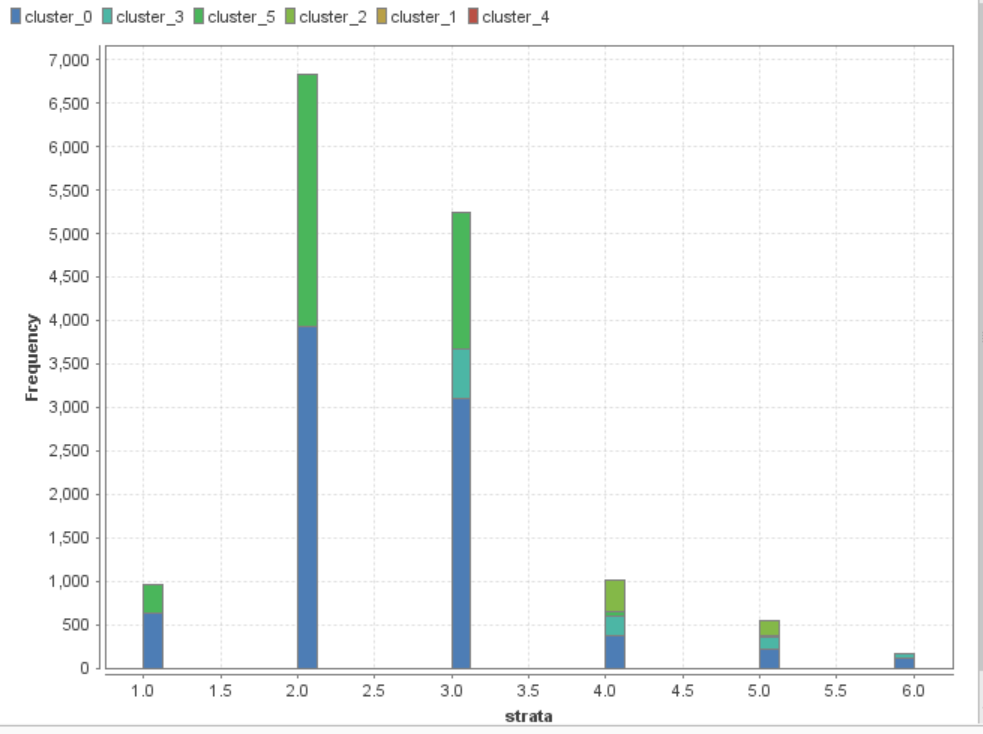
\includegraphics[width=0.9\textwidth]{../Miriam-RapidMiner/vectorClustering.PNG}

So we change the maximal stepsize to 1000 and let the algorithm run again.

\begin{figure}[h]
\centering
\begin{subfigure}{.5\textwidth}
  \centering
  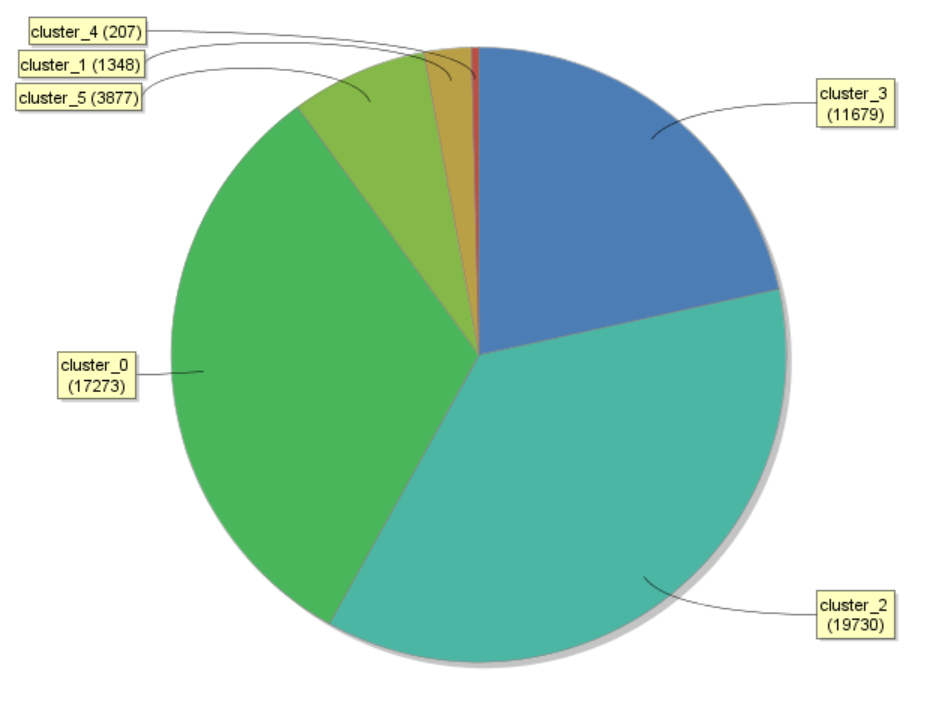
\includegraphics[width=.4\linewidth]{../Miriam-RapidMiner/vectorclusteringcluster1000.PNG}
  \caption{Strata}
  \label{fig:OrgSt}
\end{subfigure}%
\begin{subfigure}{.5\textwidth}
  \centering
  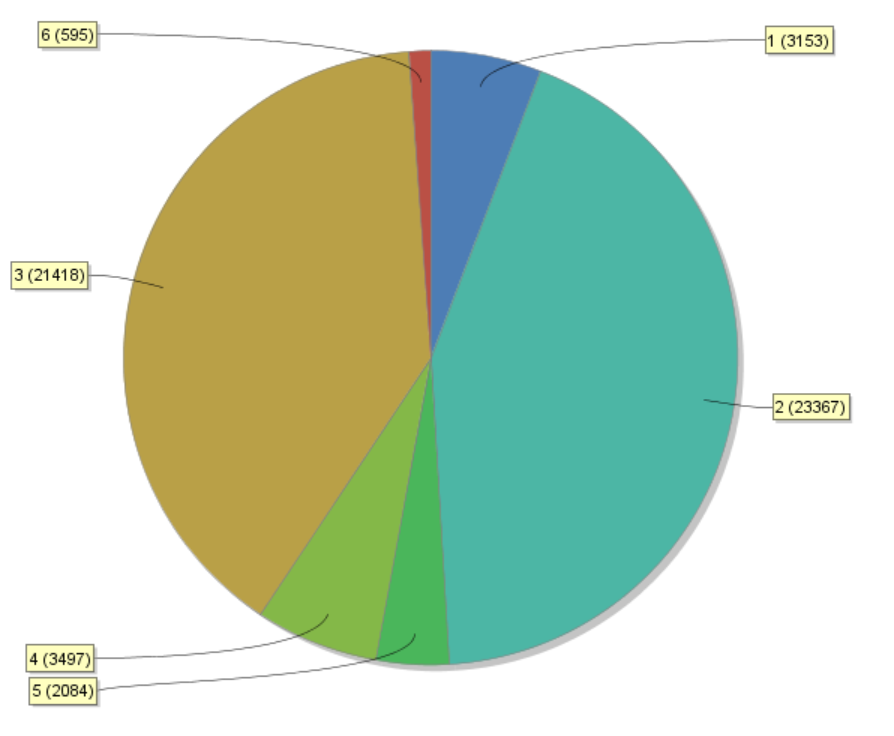
\includegraphics[width=.4\linewidth]{../Miriam-RapidMiner/vectorclusteringstrata.PNG}
  \caption{Cluster}
  \label{fig:OrgCl}
\end{subfigure}
\caption{Distribution of original data}
\label{fig:OrgDist}
\end{figure}

So we already get the idea, that there are not 6 Clusters, but just 3. Checking the distribution still gives us no strong correlation between strata and cluster.

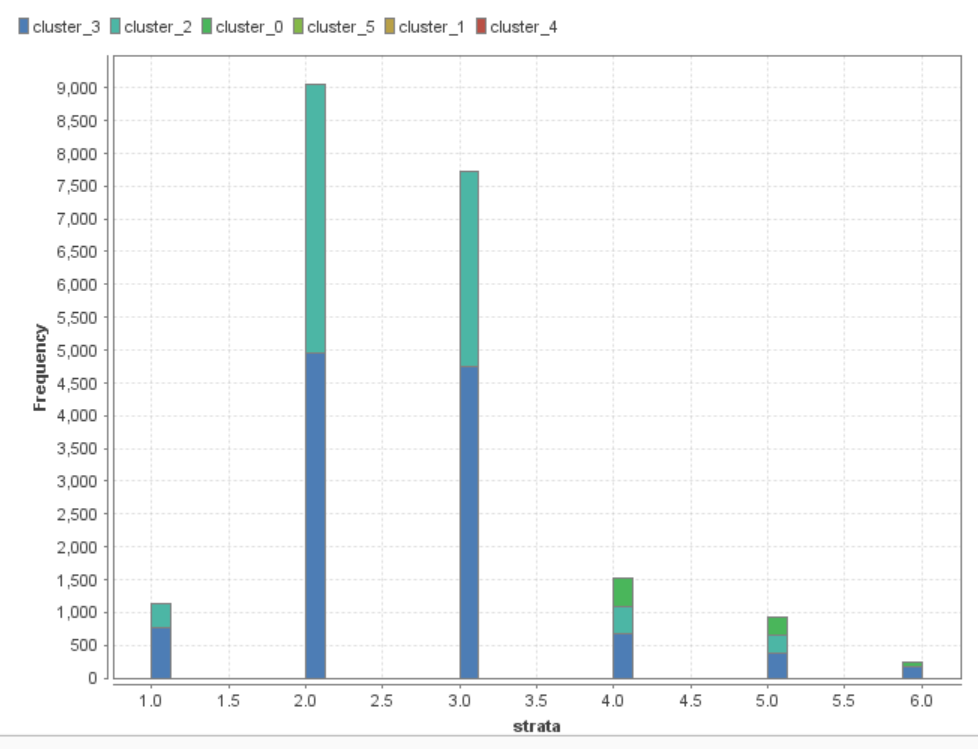
\includegraphics[width=0.9\textwidth]{../Miriam-RapidMiner/vectorClustering1000}

\subsubsection{Searching for 3 Clusters}

Because of the result in the last part, we checked the behavior of the clustering by just searching for 3 Cluster. The first try is with 100 steps again.

\begin{figure}[h]
\centering
\begin{subfigure}{.5\textwidth}
  \centering
  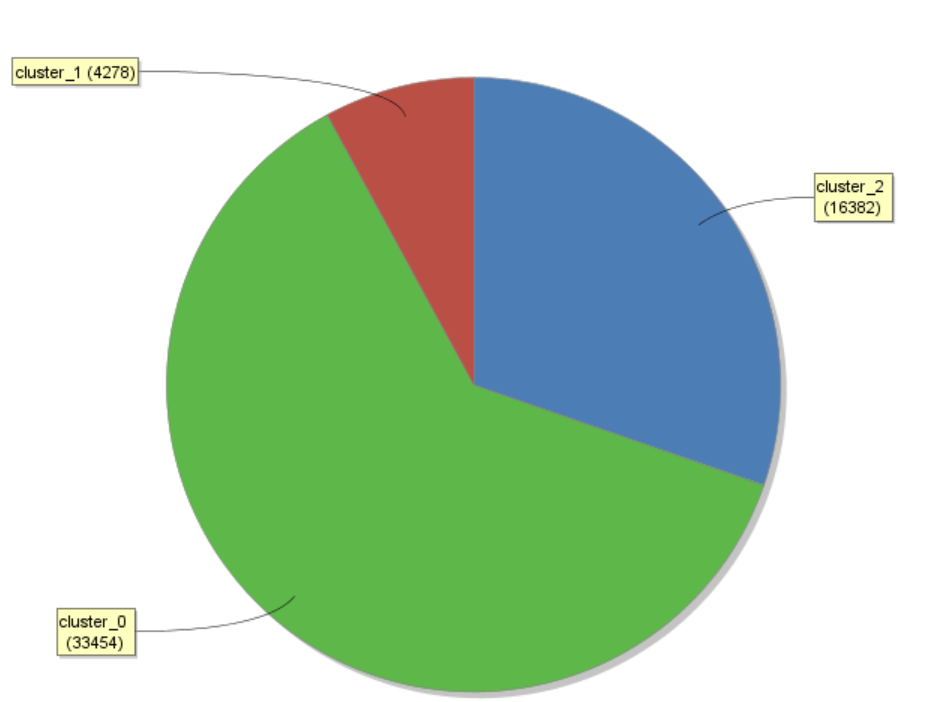
\includegraphics[width=.4\linewidth]{../Miriam-RapidMiner/vectorclusteringcluster3Cluster.PNG}
  \caption{Strata}
  \label{fig:OrgSt}
\end{subfigure}%
\begin{subfigure}{.5\textwidth}
  \centering
  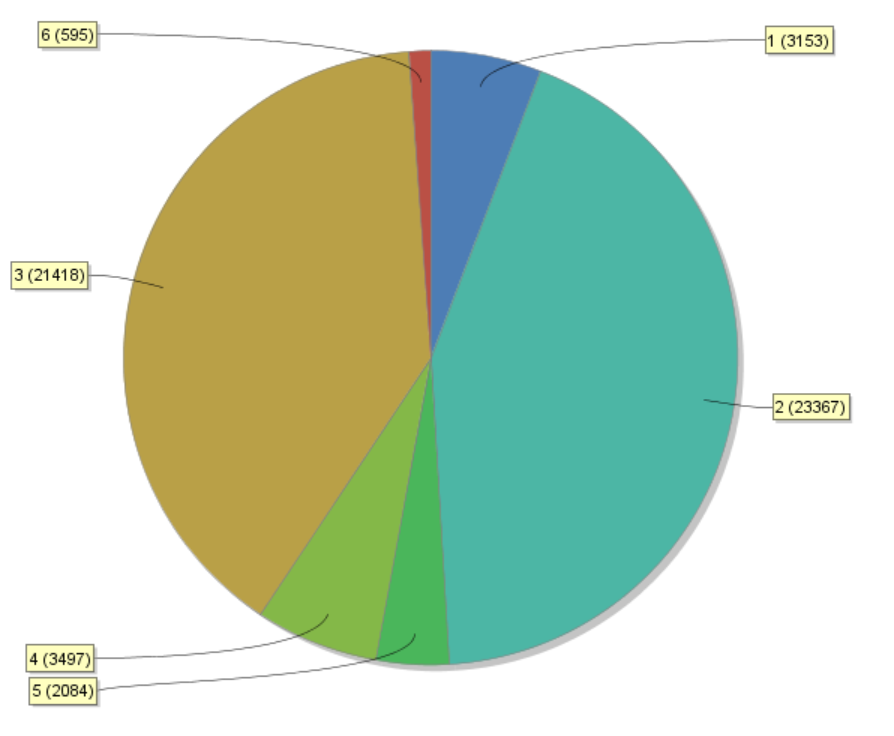
\includegraphics[width=.4\linewidth]{../Miriam-RapidMiner/vectorclusteringstrata.PNG}
  \caption{Cluster}
  \label{fig:OrgCl}
\end{subfigure}
\caption{Distribution of original data}
\label{fig:OrgDist}
\end{figure}

This comes closer by the orginial distribution combining two stratas in one cluster.

But having a look at the inbetween distribution does not show us a real correlation between cluster and strata.

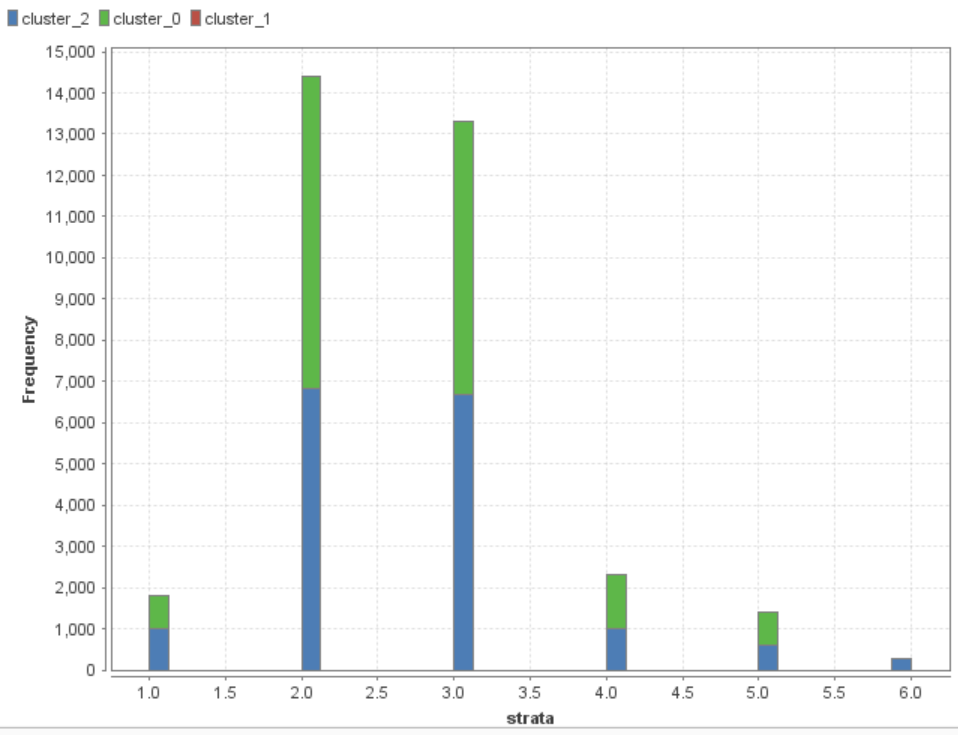
\includegraphics[width=0.9\textwidth]{../Miriam-RapidMiner/vectorClustering3Cluster.PNG}

We wanted to check what happens when giving the process 1000 steps maximal. 